\documentclass{article}
\usepackage[final]{nips_2017}
\usepackage[utf8]{inputenc} % allow utf-8 input
\usepackage[T1]{fontenc}    % use 8-bit T1 fonts
\usepackage{hyperref}       % hyperlinks
\usepackage{url}            % simple URL typesetting
\usepackage{booktabs}       % professional-quality tables
\usepackage{amsfonts}       % blackboard math symbols
\usepackage{nicefrac}       % compact symbols for 1/2, etc.
\usepackage{microtype}      % microtypography
\usepackage{graphicx}
\title{Automatic Code Generation Project Proposal}

\author{
  Lizi Ottens  \\
  Department of Computer Science\\
  Stanford University\\
  \texttt{lottens@stanford.edu}
  
  \and
  
  \textbf{Luis Perez} \\
  Department of Computer Science \\
  Stanford University \\
  \texttt{luis0@stanford.edu}
  
  \and
  
  \\
  \textbf{Sudharshan Viswanathan} \\
  Department of Computer Science \\
  Stanford University \\
  \texttt{viswans@stanford.edu}
}

\begin{document}
% \nipsfinalcopy is no longer used

\begin{center}

\includegraphics[width=3cm, height=0.7cm]{CS230}
\end{center}

\maketitle

\begin{abstract}
We propose developing a machine learning system for code generation.
\end{abstract}

\section{Problem Description}	
Automating even small parts of software development is an interesting research area \cite{survey} of machine learning that can save time for countless software engineers and resources for technology companies to invest into solving other more challenging problems. Automating code generation can take on many forms, from auto-completing lines of source code to generating lines of source code from comments, generating source code from UI images, or generating unit tests from source code. In this project, we aim to take incomplete lines of code as input and generate code to complete it. We hope that a byproduct of our endeavor will be the ability to understand and visualize \cite{visualizing_rnns} how deep learning architectures perceive and process code.

Subsequent work would be to ensure that the generated function code can compile, applying reinforcement learning to incorporate this signal in training. We also hope to extend our work to applications such as generating unit tests given a source function, or generating code given documentation. 


\section{Challenges}
A primary challenge in code generation is that it’s still an active area of research, with many possible solutions and ongoing investigation \cite{structural_code_modeling}. State of the art solutions have not yet come close to automating basic tasks software engineers perform on a daily basis.

Other challenges include restricted language domains, complexity in evaluation results, etc. Specifically, while pre-trained models are trained on free-form language data, programming languages often utilize non-natural variable names, function names, and syntax with more structure \cite{structural_code_modeling}. Work in this area has focused on creating more structured models that take advantage of specific architectures \cite{treegen}. Other approaches involve restricting the output of the model to a CFG or DSL \cite{grammar_based}. A code generation model’s output must adhere to a very specific form in order to be syntactically correct.

Compilers/interpreters could be leveraged to provide a better form of feedback and hence can be used to create labelled data, but it is left to be seen how effectively we can leverage this feedback to aid the learning process.

\section{Datasets}
We propose two approaches. The first would involve scraping open source code from GitHub. The benefits of this approach is that it would provide us with ample data to utilize, from a diverse set of open source projects. The drawback is that the data would require significant pre-processing, cleaning, and labeling.

As an alternative initial approach, we will begin with the \href{https://github.com/github/CodeSearchNet}{CodeSearchNet dataset} \cite{codesearchnet}. The dataset consists of 2 million (comment, code) pairs from open source libraries, ranging in languages from Python, Javascript, and PHP. Median code-length consists of 60-100 text tokens, with 95\% code-length of up to 350 tokens. Median documentation length consists of 10 text tokens. There also exist other curated datasets such as those used in \cite{latent_predictor_networks_for_code_generation} and \cite{learning_to_genereate_pseudo_code}.


\section{Learning Method}
Developments in the area of NLP such as GPT-2 \cite{gpt2} and BERT \cite{BERT} have significantly improved the “quality” of text generation systems. State of the art results from these models can be conditioned on a given context, encouraging the models to generate text from interesting distributions. This yields itself as a good starting point for code generation since the act of writing/reading code can be viewed as an extension of natural language. Though, such an attempt also has the additional bar of ensuring that generated code compiles, or runs on an interpreter and also produces intended outputs. 

In our project, we aim to start from pre-trained language models, and utilize that to generate code by conditioning the model and fine-tuning it to our specific task. The input to our model will be a text sequence corresponding to an incomplete function call, and the output of the model will be the completed function. 

\subsection{Code Generation}

\begin{figure}[!ht]
    \centering
    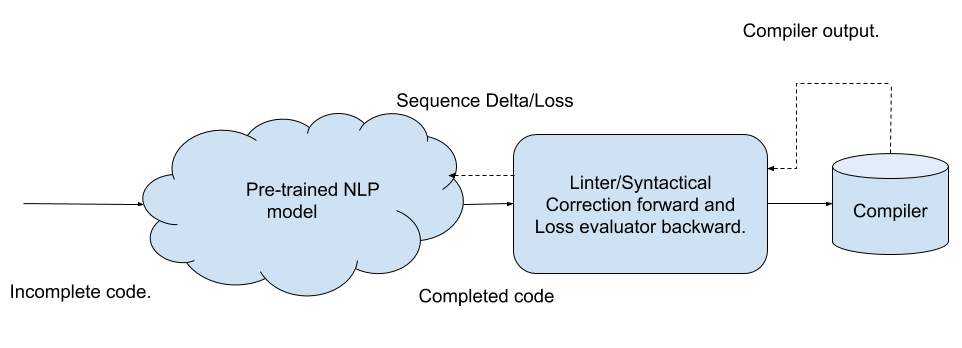
\includegraphics[scale=0.4]{auto_code_gen_diagram.png}
    \caption{Overview of Proposed Architecture for Automatic Code Generation with Compiler Feedback.}
    \label{fig:auto_code_gen}
\end{figure}

We start with a pre-trained NLP model that would generate more text that fits the context of the input. In this case, the input text is going to be code and the output would be the completed code. We would have to ensure that the generated code fits the syntax of the language and hence feed it through another network. Furthermore, the second block becomes instrumental in interpreting the compiler output and output a delta that could then be used as a loss function for the NLP model to re-evaluate its parameters. 

\subsection{Loss Computation / Adapting Compiler Feedback for Gradient Descent}
Typical software engineers use the compiler output in order to decide their next steps. And those steps would be incremental in nature. The delta change in code would serve as a very good loss function for the NLP model to train on, while the forward path of the same network could double as a linter and perform simple syntactic correction. A good way to arrive at this model would be to train different Seq2Seq models (RNN/LSTM/GRU) on known good code and randomly modify, record the delta and codify the compiler output. This would enable us to flip the model and use it to feed compiler output back into the model and generate the program delta which would serve as the loss for the first network.

\section{Evaluation}
For evaluation, we plan to hold out a fraction of the input dataset and then attempt code generation/completion on the hold out set and evaluate whether the output generated compiles in the first place, and if it does how far it deviates from the actual code that we started from. We will define a metric, compilation success rate, and report this on our generated programs. There are also other NLP-centric metrics such as the BLEU score \cite{retrieval_based_neural_code_generation} which we can use to measure how well our model outputs match the expected function.

Qualitatively, we also hope to be able to tool the networks with visualization \cite{visualizing_rnns} and extract information about what the different units encode when it comes to parsing and generating code.

\bibliographystyle{unsrt}
\bibliography{references}
\end{document}